\documentclass[10pt, a4paper]{article}

%%%%%%%%%%%%%%
%  Packages  %
%%%%%%%%%%%%%%


\usepackage{page_format}
\usepackage{special}
\usepackage{hyperref}
\usepackage{tikz}
\usepackage[compat=1.1.0]{tikz-feynman}
\input{math_func}

\usepackage{slashed}

% References
\usepackage{biblatex}
\addbibresource{ref.bib}


%%%%%%%%%%%%
%  Colors  %
%%%%%%%%%%%%
% ! EDIT HERE !
\colorlet{chaptercolor}{red!70!black} % Foreground color.
\colorlet{chaptercolorback}{red!10!white} % Background color

%%%%%%%%%%%%%%
% Page titre %
%%%%%%%%%%%%%%
\title{Homework 1} % Title of the assignement.
\author{\PA} % Your name(s).
\teacher{Francois David and Dan Wohns} % Your teacher's name.
\class{Quantum Field Theory II} % The class title.

\university{Perimeter Institute for Theoretical Physics} % University
\faculty{Perimeter Scholars International} % Faculty
%\departement{<Departement>} % Departement
\date{\today} % Date.


%%%%%%%%%%%%%%%%%%%%%%
% Begin the document %
%%%%%%%%%%%%%%%%%%%%%%
\begin{document}

% Make the title page.
\maketitlepage

% Make table of contents
\maketableofcontents

% Assignment starts here ----------------------------



\section{Gross-Neveu Model}

\begin{enumerate}
  \item[(a)] The Gross-Neveu model is a $1+1$ dimensionnal model describing a collection of $N$ fermionic fields $\psi^a$ (and a supressed Dirac index ranging from $1$ to $2$) indexed by a color index $a$ ranging from $1$ to $N$. The fermions each contribute a free massless Dirac term $\bar{\psi}_a i \slashed{\partial} \psi_a$ (summation on $a$ is implied) and are coupled with an interaction term $g^2 (\psi_a \psi^a)/(2N)$ with coupling constant $g$. The full lagrangian density reads
  \begin{align*}
    \mathcal{L}_{\mathrm{GN}}=\bar{\psi}_a i \slashed{\partial} \psi^a+\frac{g^2}{2 N}\left(\bar{\psi}_a \psi^a\right)^2. 
  \end{align*}
  We work in natural units where $\hbar = 1, c = 1$ making all quantitities of interest gain dimension of a power of mass. For action, length and time these powers are respectively $0$, $-1$ and $-1$. Since the action is dimensionless and obtained by integrating the lagrangian density $\mathcal{L}_{\mathrm{GN}}$ over $1+1$ spacetime dimensions, we have $0 = [\mathcal{L}_{\mathrm{GN}}] +  [dx^2] = [\mathcal{L}_{\mathrm{GN}}] - 2 \implies [\mathcal{L}_{\mathrm{GN}}] = 2$. Knowing the dimension of the lagrangian density, we use the kinetic term to compute the dimension of the fields. Since the derivatives have the inverse dimension of their associated variables, we have $2 = 2[\psi^a] + [\slashed{\partial}] = 2[\psi^a] + 1 \implies [\psi^a] = 1/2$. Finally, the dimension of the coupling constant can be extracted using the interaction term. Indeed,  $2 = 4 [\psi^a] + 2 [g] = 2 + 2 [g] \implies [g] = 0$ making the coupling constant dimensionless. 
  \item[(b)] The slashed derivative $\slashed{\partial}$ appearing in the lagrangian density is the result of a contraction of the $\gamma^\mu = (\gamma^0, \gamma^1)$ with the partial derivatives $\partial_\mu = (\partial_0, \partial_1)$. In $1+1$ dimensionnal spacetime we can form a clifford algebra with $\gamma^0 = \sigma^2, \gamma^1 = i \sigma^1$ where $\sigma^2, \sigma^1$ are Pauli matrices. We also have $\gamma^5 = \gamma^0 \gamma^1 = \sigma^3$. Following the properties of clifford algebras, we have that $\gamma^5$ anticommutes with all $\gamma^\mu$ matrices. All the $\gamma^\mu$ matrices are multiplied together in $\gamma^5$ and any $\gamma^\mu$ commutes with itself, but anticommutes with the remaining matrix in the product leading to $\{\gamma^5, \gamma^\mu\} = 0$. The Dirac adjoint of the fermionic fields appearing in the lagrangian density is defined to be $\bar{\psi}_a = \psi^{a\dagger} \gamma^0$.  We relate $\psi^{a}$ and a transformed field $\phi^{a}$ by $\psi^{a} = \gamma^5 \phi^{a}$. In terms of the transformed field, the  Dirac adjoint of $\psi^{a}$ becomes $\bar{\psi}_a = \phi^{a\dagger}\gamma^{5\dagger} \gamma^0 = -\phi^{a\dagger} \gamma^0 \gamma^{5} = -\bar{\phi}_a \gamma^5$ because $\gamma^5 = \sigma^3$ is real. Using these expressions, we can express $\mathcal{L}_{\mathrm{GN}}$ in terms of the transformed field as follows: 
  \begin{align*}
    \mathcal{L}_{\mathrm{GN}}=-\bar{\phi}_a \gamma^5 i \slashed{\partial} \gamma^5 \phi^a+\frac{g^2}{2 N}\left(-\bar{\phi}_a \gamma^5 \gamma^5 \phi^a\right)^2 = \bar{\phi}_a i \slashed{\partial}  \phi^a+\frac{g^2}{2 N}\left(\bar{\phi}_a \phi^a\right)^2  
  \end{align*}
  where we used $\{\gamma^5, \gamma^\mu\} = 0$ in the first term and $\gamma^5 = 1$ in the second term. We notice that the new lagrangian density is identical to the $\psi^a$ one and the transformation from $\psi^a$ to $\phi^a$ is a discrete symmetry. A mass $m$ term $m \bar{\psi}_a \psi^a$ would transform to $-m \bar{\phi}_a \gamma^5 \gamma^5 \phi^a = -m \bar{\phi}_a \phi^a$ which is not identical to the initial term and therefore breaks the considered symmetry. 
  \item[(c)] The interaction term implies that the scattering amplitudes can be computed using Feynman digragmatic for a $4$ particle vertex. Expanding the square of the interaction term we see that the vertex involves one (self-interaction) or two colors. For each color, it has an ingoing fermion and an outgoing fermion (arising from wick contractions with $\bar{\psi}_a$ and $\psi^a$). The coefficient of each term in the expansion is $g^2/N$ because the factor of $2$ is canceled by the binomial coefficient of the square expansion. We are interested in the two point function $\langle \bar{\psi}_b \psi_a\rangle$. At on loop order the only there is only one vertex and it has two of its fields contracted together to close the loop. The only non-vanishing one-loop contribution contracts fields sharing the same type and the effective interaction term is of the form $\bar{\psi}_a \psi^a \bar{\psi}_a \psi^a$ (with no summation implied). This implies that the incomming and outgoing fields are contracted with the same color forcing them to share this color. Therefore, the one-loop correction only consitutes a self-interaction correction. The position space diagram associated to this process and its amplitude are 
  \begin{equation*}
    \langle \bar{\psi}_a \psi_a \rangle_{\text{one \ loop}} = 
    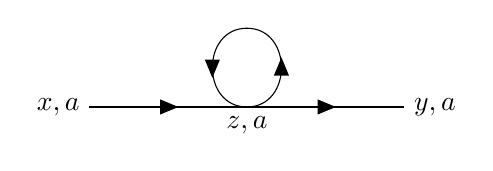
\begin{tikzpicture}[baseline=(current bounding box.center)]
      
      \begin{feynman}
        % External legs

        \vertex[label={left:$x, a$}]  (a) at (-2, 0);
        \vertex[label={right:$y, a$}] (b) at (2, 0);

        \vertex[label={below:$z, a$}]  (p) at (0, 0);
        \vertex (q) at (0, 1); 

        %\fill (a) circle (2pt);
  
        \diagram* {
          (a) --[fermion] (p),
          (p) --[fermion] (b),
          (p) --[fermion, half right] (q),
          (q) --[fermion, half right] (p),
        };
      \end{feynman}
    \end{tikzpicture}
    = -i \frac{g^2}{\hbar N} \int \ \text{d}^4 z \  \hbar (\slashed{\partial})^{-1}_{xz} \hbar (\slashed{\partial})^{-1}_{zz} \hbar (\slashed{\partial})^{-1}_{zy}
  \end{equation*} 
  where $(\slashed{\partial})^{-1}_{xz}$ denotes the free massless fermionic propagator between points $x$ and $z$. We note that the amplitude takes the form of a matrix in spinor index consistently with the supressed spinor indices in $\langle \bar{\psi}_a \psi_a \rangle_{\text{one \ loop}}$.
  \item[(d)]
  \item[(e)]
  \item[(f)] 
  \item[(g)]
  \item[(h)]
\end{enumerate}



\section{Acknowledgement}
I worked on my own for this assignment.


% References
\makereferences
%-------------------------------------------------------


%%%%%%%%%%%%%%%%%%%%%%%%
% Terminer le document %
%%%%%%%%%%%%%%%%%%%%%%%%
\end{document}